\documentclass[avery5371, grid,frame]{flashcards}

\usepackage{graphicx}
\usepackage{geometry}

\geometry{a4paper, landscape, margin=0.2in}
\cardfrontstyle[\large\slshape]{headings}
\cardbackstyle{empty}

\begin{document}

\renewcommand{\cardpaper}{a4paper}
\renewcommand{\cardpapermode}{landscape}
\renewcommand{\cardrows}{2}
\renewcommand{\cardcolumns}{2}
\setlength{\cardheight}{3.5in}
\setlength{\cardwidth}{5.0in}
\setlength{\topoffset}{0.50in}
\setlength{\oddoffset}{0.50in}
\setlength{\evenoffset}{0.50in}

\begin{flashcard}{check}
    \vspace*{\fill}
    \begin{center}
        \begin{minipage}[c]{.45\textwidth}
            
\includegraphics[width=\textwidth]{cards/c/check/check - a detective with a magnifying glass closely examining a document, searching for clues.png}
        \end{minipage}
        \begin{minipage}[c]{.45\textwidth}
            \begin{itemize}\setlength\itemsep{12pt}
            \item Explanation: \ To look carefully to find mistakes or problems

            \item Example: \ a detective with a magnifying glass closely examining a document, searching for clues
            \end{itemize}
        \end{minipage}
    \end{center}
    \vspace*{\fill}
\end{flashcard}\begin{flashcard}{check}
    \vspace*{\fill}
    \begin{center}
        \begin{minipage}[c]{.45\textwidth}
            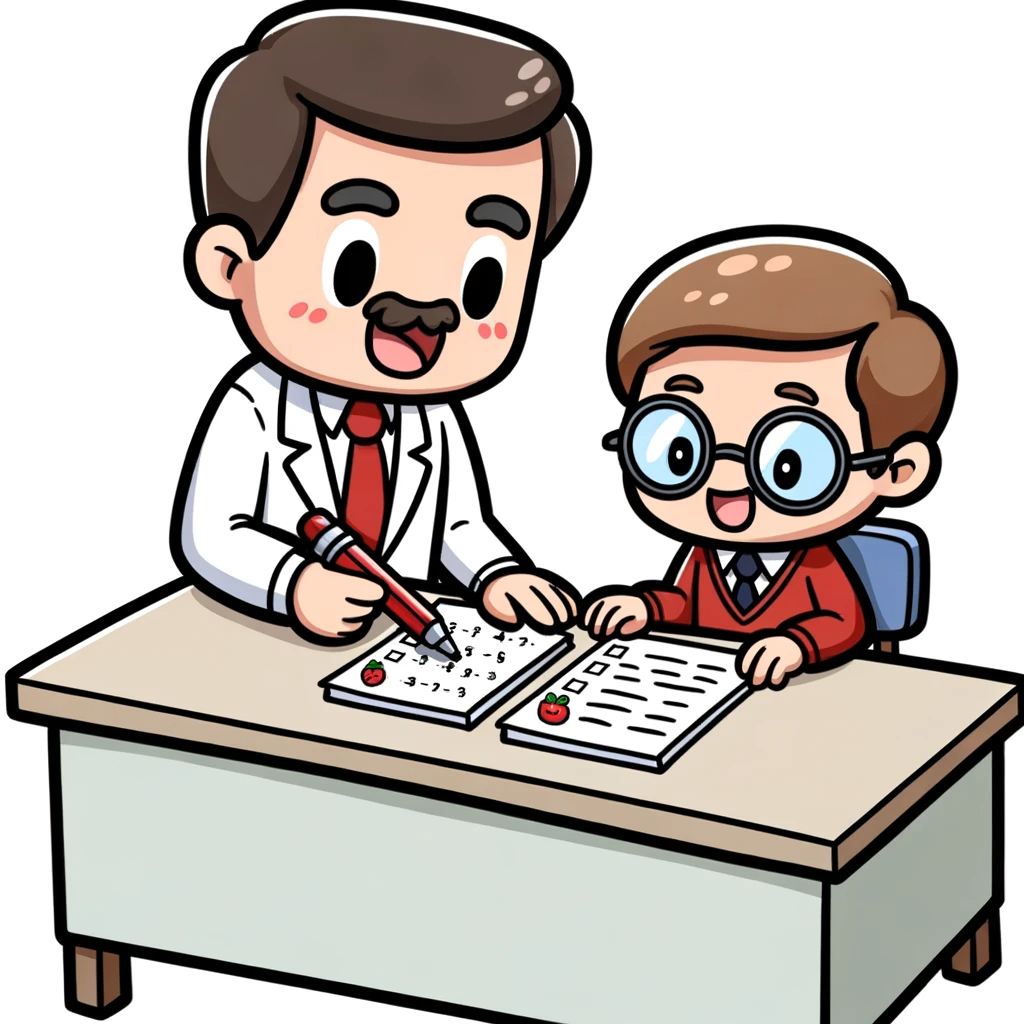
\includegraphics[width=\textwidth]{cards/c/check/check - a teacher with a red pen, reviewing a student's homework on a desk, looking for errors.png}
        \end{minipage}
        \begin{minipage}[c]{.45\textwidth}
            \begin{itemize}\setlength\itemsep{12pt}
            \item Explanation: \ To look carefully to find mistakes or problems

            \item Example: \ a teacher with a red pen, reviewing a student's homework on a desk, looking for errors
            \end{itemize}
        \end{minipage}
    \end{center}
    \vspace*{\fill}
\end{flashcard}\begin{flashcard}{check}
    \vspace*{\fill}
    \begin{center}
        \begin{minipage}[c]{.45\textwidth}
            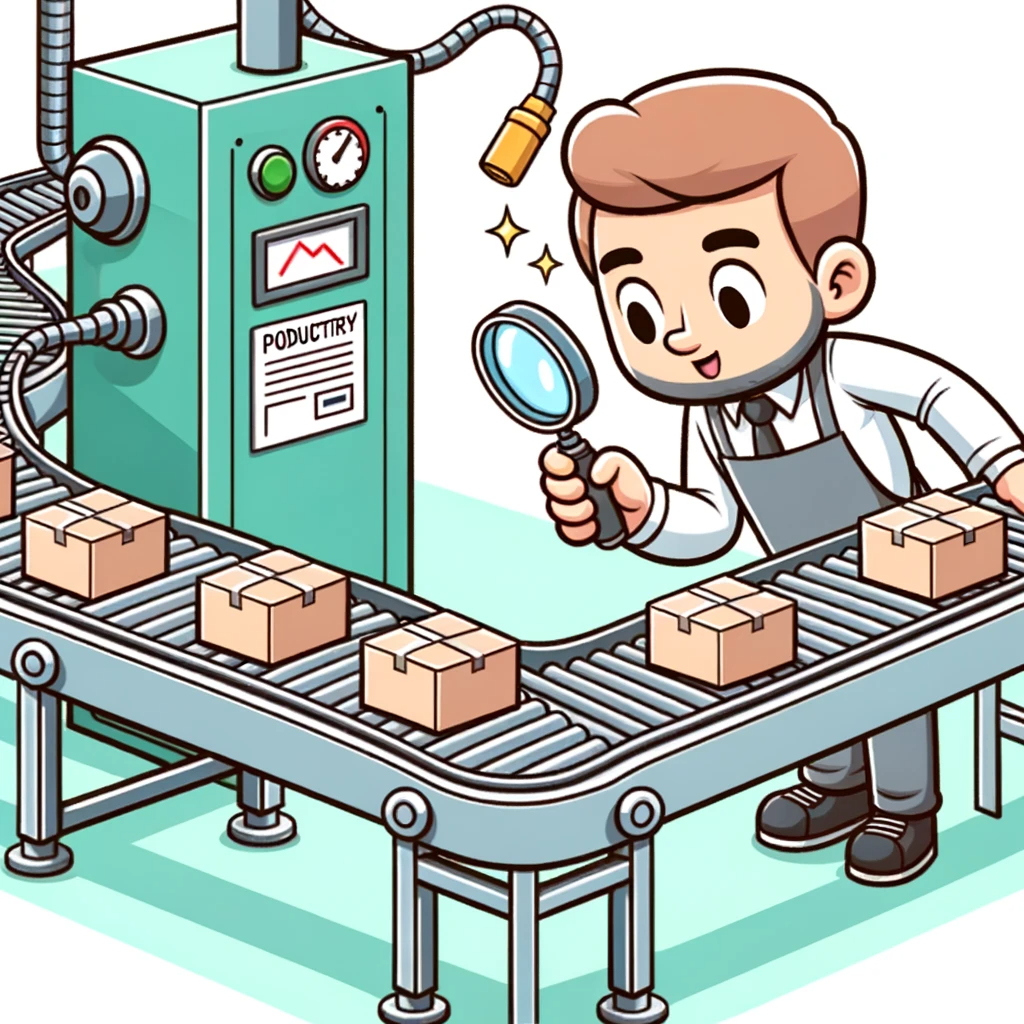
\includegraphics[width=\textwidth]{cards/c/check/check - a worker at a factory conveyor belt, inspecting products and ensuring their quality.png}
        \end{minipage}
        \begin{minipage}[c]{.45\textwidth}
            \begin{itemize}\setlength\itemsep{12pt}
            \item Explanation: \ To look carefully to find mistakes or problems

            \item Example: \ a worker at a factory conveyor belt, inspecting products and ensuring their quality
            \end{itemize}
        \end{minipage}
    \end{center}
    \vspace*{\fill}
\end{flashcard}\begin{flashcard}{check}
    \vspace*{\fill}
    \begin{center}
        \begin{minipage}[c]{.45\textwidth}
            
\includegraphics[width=\textwidth]{cards/c/check/check - a computer programmer staring intently at a computer screen, debugging lines of code.png}
        \end{minipage}
        \begin{minipage}[c]{.45\textwidth}
            \begin{itemize}\setlength\itemsep{12pt}
            \item Explanation: \ To look carefully to find mistakes or problems

            \item Example: \ a computer programmer staring intently at a computer screen, debugging lines of code
            \end{itemize}
        \end{minipage}
    \end{center}
    \vspace*{\fill}
\end{flashcard}

\end{document}